\documentclass[11pt]{article}
\usepackage[letterpaper,hmargin=1in,vmargin=1.25in]{geometry} 
\usepackage{graphicx}                   % graphics (includegraphics)
\usepackage{url}                        % \url{...} formatting URLs
\usepackage[dvipsnames]{xcolor}         % colored text and backgrounds
\usepackage{hyperref}                   % add hyper-references
\usepackage{listings}
\usepackage{titlesec}
\titlelabel{\thetitle.\quad}
\titleformat*{\section}{\bfseries}
\lstset{%
	basicstyle=\ttfamily,
	breaklines = false,
	tabsize=2
}
\begin{document}
	
	\begin{center}
		\large\textbf{U.S. Digital Corps | 2024 Software Engineering Project-Based Assessment}
		\\\textbf{Raion Fet}
	\end{center}
	
	\hspace*{-0.6cm}\textbf{\\Overall process and decision making:}
	\normalfont {
		\\Before starting development, I wanted to first understand what were the desired requirements and goals of the assessment as well as setup the necessary pieces for final assessment delivery. Therefore, instead going straight into coding, I spent time reading over the provided assessment instructions to ensure I fully understood how to proceed with the development process as well as determine what was necessary to start and complete the assessment. 
		\\\\In more detail, I created a public Git repository based on the submission standards and example practice repository provided in the assessment document, then I used TeXstudio to create and format the .pdf file that will have all the written responses based on the assessment requirements, and also set up the Visual Studio coding environment that I was going to use to work on development. While the document specified that the assessment repository should mainly contain the tester.html and book\_search.js files, I also included a folder with all the TeX related files and documentation so that all the aspects of the assessment would be contained in one place and were easily accessible. By completing these steps, it made the development and submission process more straightforward because all of the administrative duties and requirements had already been taken care of.
		\\\\Now I was able to begin the development process. I first wanted to understand the overall template and structure of the JSON object that the findSearchTermInBooks function would be taking in and working with. To do this, I analyzed the example JSON object input provided in book\_search.js to understand the object and its fields as a whole. By understanding the object in its entirety I can visualize how I should develop the process that searches through the object using easily identifiable logic and literally named variables. Using easy to understand logic and variables names based on the JSON object allows any individual to follow the code without difficulty. More importantly, it also allows me to go back and look over code that I have previously developed and understand it with a quick glance over.
		\\\\Going back to the process of analyzing the JSON, I realized that while the example input object is described to have one book and its related contents, as a whole, the JSON can contain zero or more books since it is an array of books and its respective fields. Therefore, the JSON object is more akin to a library with a list of books that can have any amount of desired contents. This visualization is clearly represented in Figure 1.
		
		\begin{figure}[htbp]
			\centerline{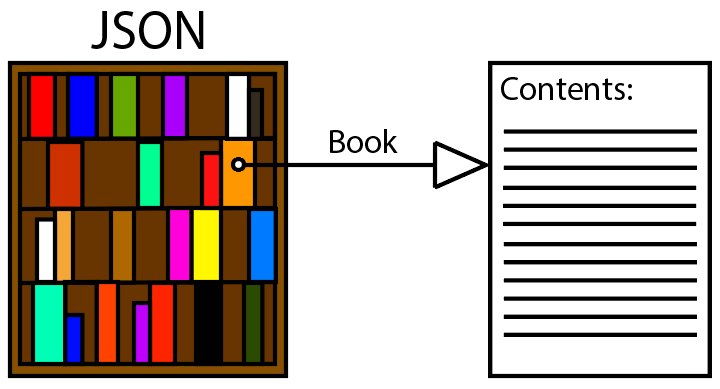
\includegraphics[scale=0.45]{Diagrams/Diagram1}}
			\caption{JSON visualization.}
		\end{figure}
		
		\pagebreak
		\hspace*{-0.6cm}Once the JSON object was fully comprehended, I could start coding the process that I had initially visualized. In more detail, the function should start by searching through all of the books one by one. For each book, the function must also search the list of contents and determine if the text within that content contains the search word provided to the function. Overall, the function at this point contains two looping processes that search the book and its respective contents for the desired search term. 
		\\\\Now to complete the function and achieve the desired goals for the assessment, it was necessary to analyze the overall template and structure of the function's return value. To do so, I repeated the process for comprehending the JSON object input. 
		\\\\More particularly, I looked over the example output object in book\_search.js and understood that the desired output for the findSearchTermInBooks function was a JSON object that contained the provided search term and a list of all the book content that contained that search term. Therefore, at every function call, a resulting JSON object must be created whether or not a match is found and that's because the search term is a value that will always exist. However, the results list of the returned JSON object may or may not contain a populated list because of the aforementioned possibilities of a match. 
		\\\\After this analysis, I completed the function by initializing a JSON return value at every function call and immediately put the value for the object's search term. Furthermore, within the secondary process of searching through a book's contents, if the search word is determined to be found within the text of a book's content, then the book's ISBN and it's content line and page is added to the list of results. 
		\\\\By making all of these decisions, the findSearchTermInBooks function should be able to search over any number of books and return a JSON object that has all the content that matches a provided search term, completing the implementation goal of the assessment.
	}
	
	\pagebreak
	\hspace*{-0.75cm}\textbf{
		Testing and iteration:
	}
	\textbf{\\i. }\normalfont{
		When it came to creating the unit tests, the main things I wanted to test were whether the function returned the correct output for an empty JSON, a JSON with books but empty content, a JSON with a single book and multiple books, and could differentiate between uppercase and lowercase search terms. Therefore, my main strategy was ensuring that the function worked properly for a scanned object with zero or more books, whether there were zero or multiple matches. \\\\If I had more time to work on this problem, I would try to make the test suite more robust by automating the JSON object generation so that the function could be tested with a varying number of books and content.
	}
	\\\\\textbf{ii. }\normalfont{
		While I wouldn't say my solution is the most groundbreaking or optimal implementation, I am proud of how straightforward the solution is. My implementation is simply search the JSON for books and for each book, determine if there is any text in the list of contents that contain the search term. \\\\Another part of the solution that I'm proud about are the variables that are named literally based off the JSON input object. For example, in the first iterative process, the function gets a book which allows it to view its bookContents then view its contentSections which may contain text matching the search term. 
		\\\\The clear logic of the implementation and the variable names, not only help me in quickly understanding any code that I look back on but it also helps when any other individual has to look over and understand my code as well.
	}
	\\\\\textbf{iii. }\normalfont{
		The part of the problem that was the most difficult to solve was comprehending the JSON input object to start the development process. I would say this was the most difficult part of the problem because without fully understanding the input object, it would be impossible to create a logical implementation for the findSearchTermInBooks function.
	}
	\\\\\textbf{iv. }\normalfont{
		The main edge cases I addressed in my code were empty JSON input objects, a JSON object with empty content, using case sensitive search terms, and testing the function with an empty string search term. If I had more time to work on this problem, the main edge cases would be related to testing larger JSON objects. These objects could possibly have lengthier forms of content which would allow me to determine how the function would react or interact with different variations of data.
	}
		
\end{document}